\documentclass{article}
\usepackage{geometry}
\geometry{legalpaper, margin=1in}
\usepackage[utf8]{inputenc}
\usepackage{hyperref}
\usepackage{graphicx}
\hypersetup{
    colorlinks=true,
    linkcolor=blue,
    filecolor=magenta,
    urlcolor=cyan,
}


\title{User Manual for the InifiniTag Document Tagging Service}
\author{Barnhill, Hanif, Vinokour, Wich, Sakib, Daudrich, Sippl}
\date{Juli 2020}

\begin{document}

\maketitle
\tableofcontents

\newpage

\section{Introduction}
This documentation is aimed at the user attempting to use the InfiniTag software. The prerequesites
for this documentation are:

\begin{enumerate}
    \item The Solr database has already been setup
    \item The back end has been installed with the requirements
    \item The front end has been setup and is running.
\end{enumerate}

\bigskip
\noindent
For instructions on getting the front and back ends set up, see the \href{https://github.com/AMOS-5/infinitag/blob/master/README.md}{README} in the repository.

\bigskip
\noindent
For help getting the Solr database up and running. See the various files in our \href{https://github.com/AMOS-5/infinitag/tree/master/docs/solr}{Solr documentation}.



\section{Start Page}
\label{docoverview}

Once the front end is up and running, navigate to the start page to see a dashboard as seen in Figure \ref{fig:start_page} giving you a some statistics about the state of your documents and keyword models.

Notice in the top right corner is a status badge indicating the connection to the back end. If this is 'DOWN', then you will not be able to send or receive information from the server and will not be able to continue.
Right next to it is a language option, which allows you to use our software in both english and german, whatever you prefer.

At the bottom of the page you can see a wordcloud of all currently applied keywords, providing you with a quick and easy way to see what keywords are used often and how many there are total.

\begin{figure}
    \centering
    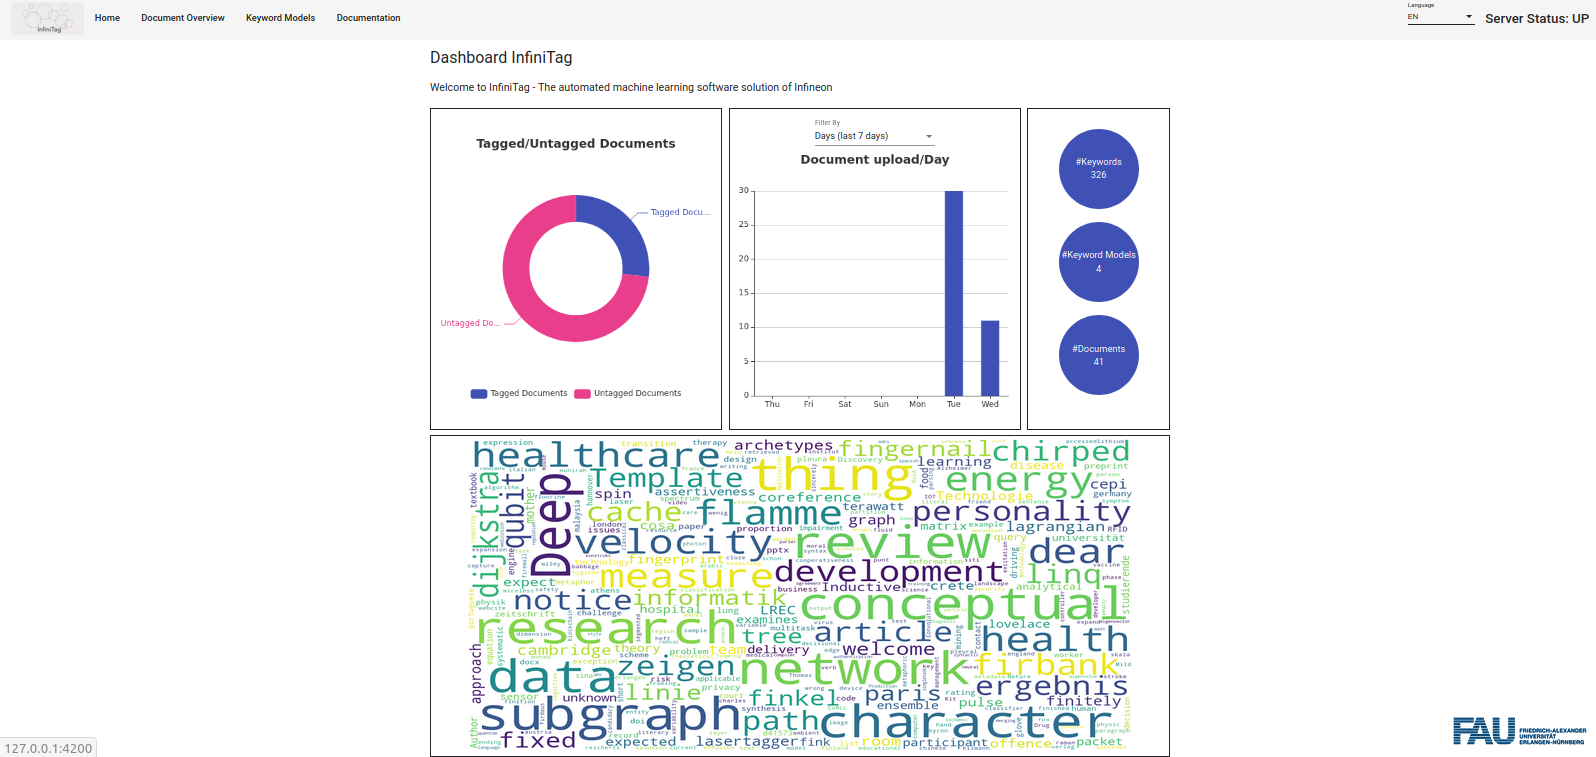
\includegraphics[scale=0.25]{img/dashboard.png}
    \caption{The Start page}
    \label{fig:start_page}
\end{figure}


\section{Document Overview}

By clicking on the Document Overview tab in the toolbar you can navigate to the page showing you all documents in the database as seen in Figure \ref{fig:doc_overview}.
The files can be sorted by their attributes by clicking on the respective label. At the top of the page is a search bar allowing you to filter files by a search term.
As the default every field in the database gets searched for the entered term, which also includes the documents name and content.
If you only want to search for specific tags you can press the Search keywords only checkbox.
In addition to that you can filter documents by their last edited timestamp by clicking on the Search By Date Range field.

You can upload more files by dragging them into the designated area marked blue or open a file dialog by clicking on it.
A dialog will open ahowing you the upload status as well as giving you an option to cancel the upload.

Keywords can be added to documents by clicking on the + sign in the MyKeywords column and can be deleted by pressing the x next to the keyword.
If you wish to add/delete multiple keywords to/from multiple documents at once, you can do so by selecting the Tagging tab.
A checkbox will become visible next to each document and you can enter multiple keywords into field titled Search Keywords....
Then the selected keywords can be applied or deleted by pressing the respective button.

In the Tagging tab you can use our automated taggin solution, too. We provide two ways to automatically tag your documents. They can be choosen by selecting them from the drop down menu on the right.
The first one tags documents by utalising something we call keyword models. Keyword models will explained in detail later in the Section \ref{}.
The second method is completly automated. You only need to select the documents or click the Apply to all documents button and typing in the amount of clusters and keywords you want.
The result of all tagging methods can be seen in Figure \ref{fig:applied_kw}. Notice how the keywords are color coded indicating by which method they were created.

If you want to download a document you can do that by clicking on the documents title or you can download multiple files at once by navigating to the Download/Delete tab.
If you download a couple of files at once, they are combined into a zip file for your convenience. In this tab you can also delete files from the database if you don't need them anymore.

\begin{figure}
    \centering
    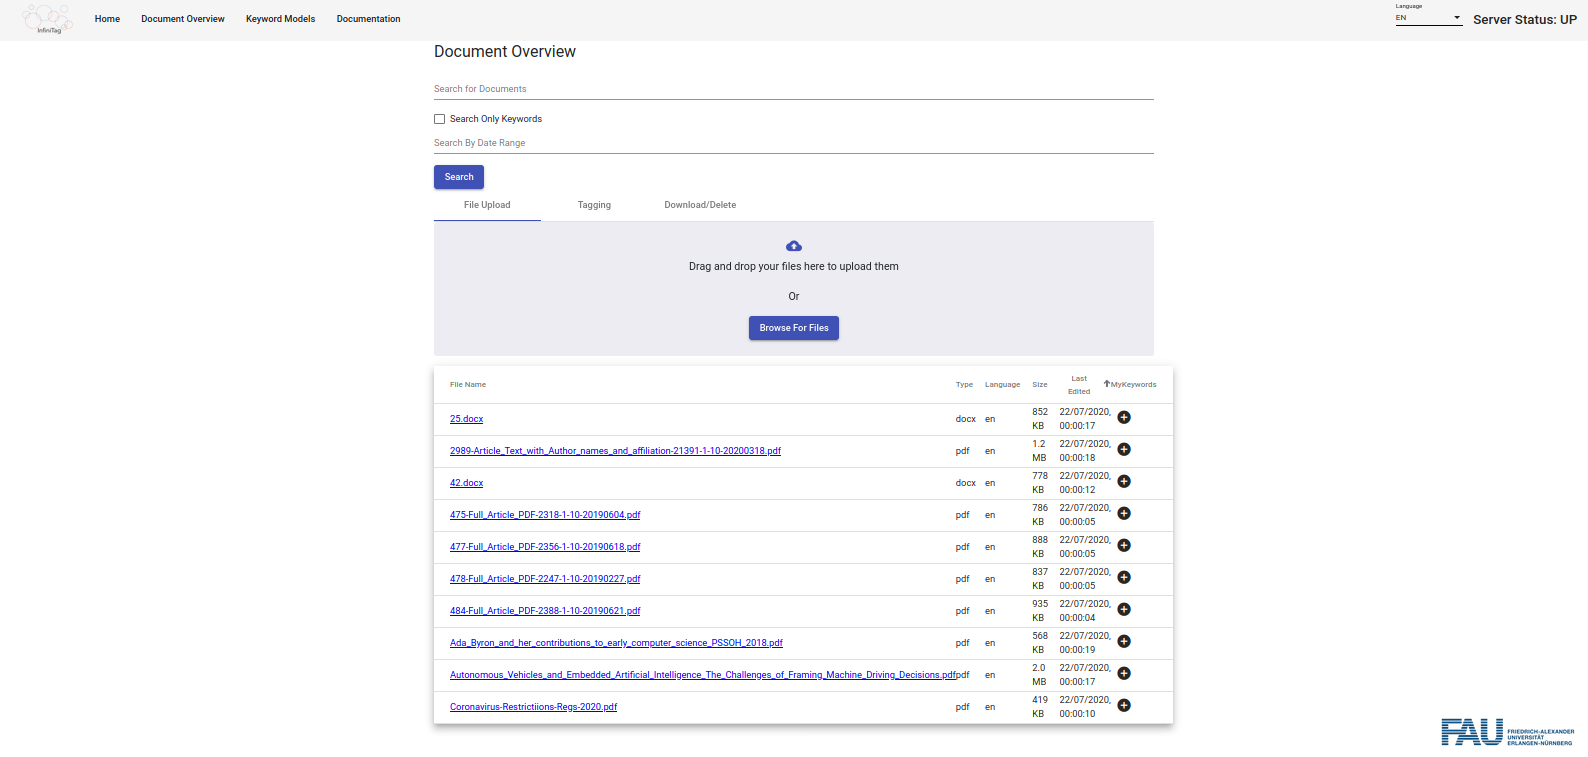
\includegraphics[scale=0.25]{img/doc1.png}
    \caption{The Document Overview}
    \label{fig:doc_overview}
\end{figure}

\begin{figure}
    \centering
    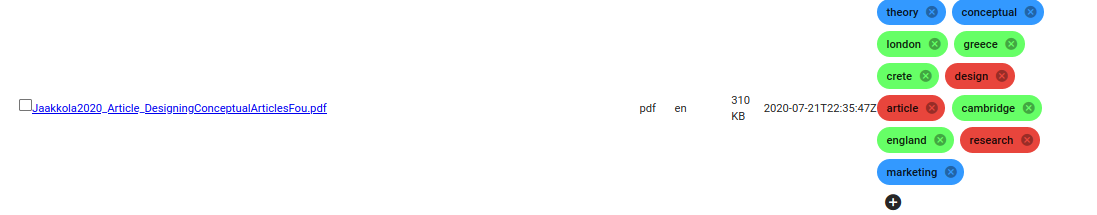
\includegraphics[scale=0.25]{img/applied_kw.png}
    \caption{Keywords applied to a document}
    \label{fig:applied_kw}
\end{figure}

\section{Keyword Models}
Navigating to \verb|keywords| or clicking on the \verb|Keywords| link will take the user to a page where they can add dimensions and keywords to a keyword model as seen in Figure \ref{fig:key1}. These keywords are then available to be assigned to the documents on the start / document overview page.

Here one can add dimensions as well as keywords, which will enable the construction of hierarchical keyword models.

\begin{figure}
    \centering
    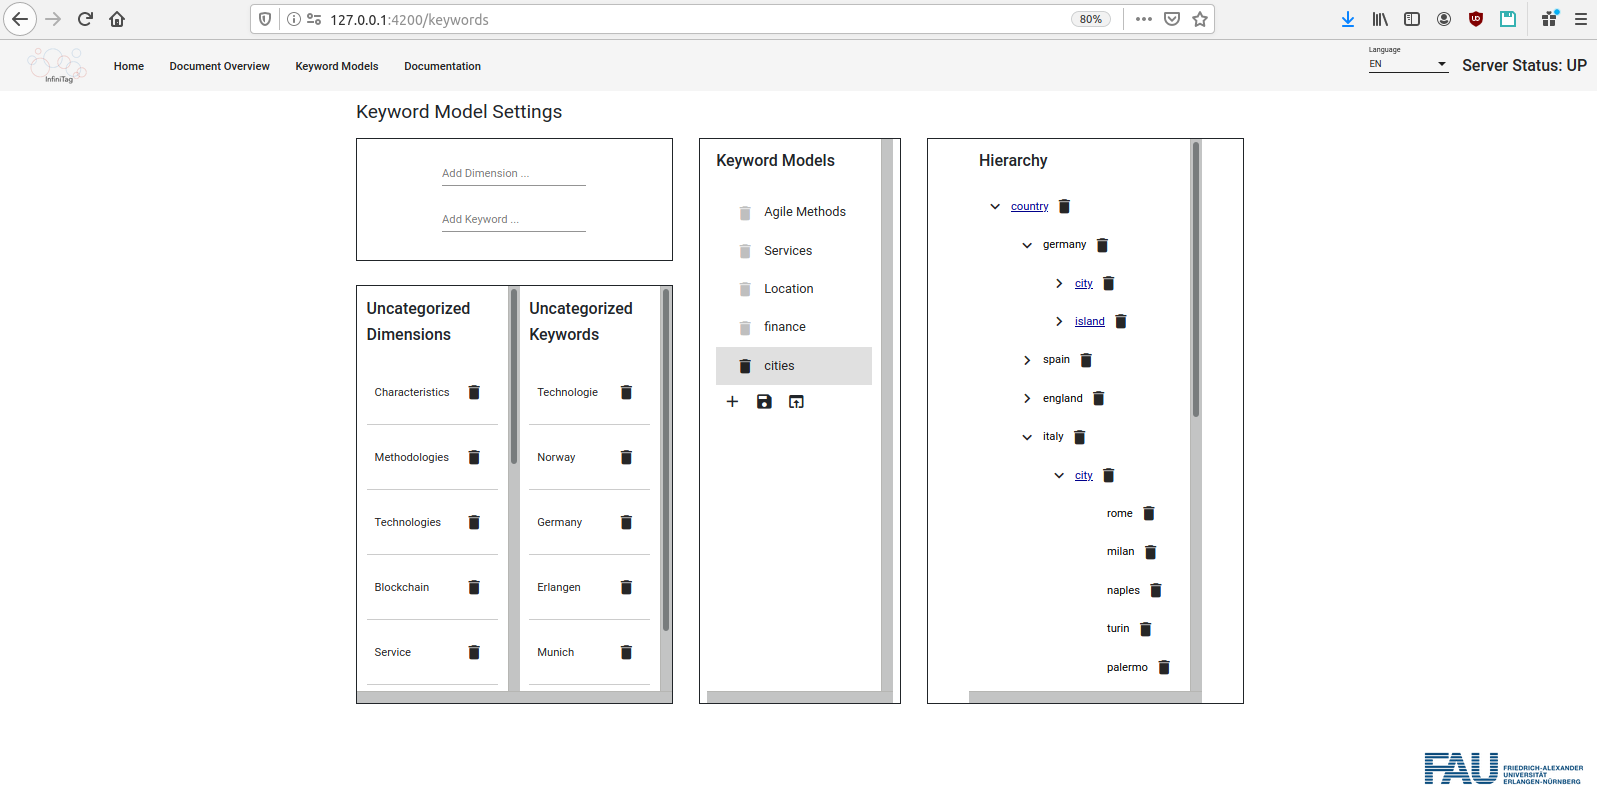
\includegraphics[scale=0.4]{img/key1.png}
    \caption{Maintaining Keywords}
    \label{fig:key1}
\end{figure}

\section{Further Documentation}
Clicking on the \verb|Documentation| link will provide the user with three options as seen in Figure \ref{fig:doc_drop}:

\begin{enumerate}
    \item API Documentation. This provides the user with an overview of all API endpoints for the back end, along with the required parameters and expected return results. A partial example can be seen in Figure \ref{fig:apidoc}
    \item Front End Documentation. This is an external link which will show the user the actual code documentation for the front end.
    \item Back End Documentation. This is another external link which will show the code documentation for the server.
\end{enumerate}

\begin{figure}
    \centering
    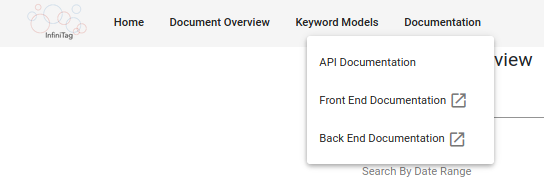
\includegraphics[scale=0.4]{img/doc3.png}
    \caption{Documentation Drop Down}
    \label{fig:doc_drop}
\end{figure}

\begin{figure}
    \centering
    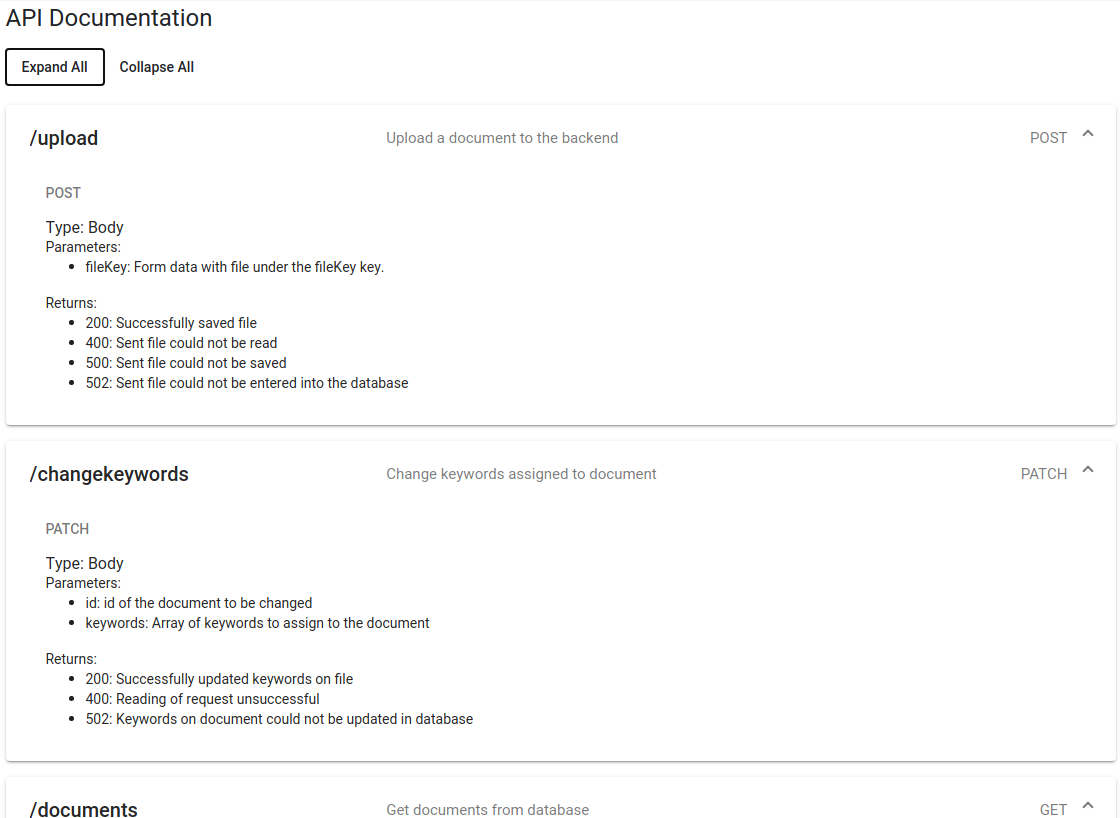
\includegraphics[scale=0.4]{img/api1.png}
    \caption{API Documentation}
    \label{fig:apidoc}
\end{figure}


\section{Utilities}
Important to notice is that the InfiniTag software comes with a utils folder. These are, in part, helper functions for the developers. However much more importantly are the scripts for categorizing and clustering documents. These scripts provide functionality for k-means clustering, hierarchical clustering, LDA, and TF-IDF. These are experimental features which will be integrated into the core solution as soon as possible.

\section{License}
InfiniTag Copyright © 2020 AMOS-5
Permission is hereby granted,
free of charge, to any person obtaining a copy of this software and
associated documentation files (the "Software"), to deal in the Software
without restriction, including without limitation the rights to use, copy,
modify, merge, publish, distribute, sublicense, and/or sell copies of the
Software, and to permit persons to whom the Software is furnished to do so,
subject to the following conditions: The above copyright notice and this
permission notice shall be included in all copies or substantial portions
of the Software. THE SOFTWARE IS PROVIDED "AS IS", WITHOUT WARRANTY OF ANY
KIND, EXPRESS OR IMPLIED, INCLUDING BUT NOT LIMITED TO THE WARRANTIES OF
MERCHANTABILITY, FITNESS FOR A PARTICULAR PURPOSE AND NONINFRINGEMENT. IN
NO EVENT SHALL THE AUTHORS OR COPYRIGHT HOLDERS BE LIABLE FOR ANY CLAIM,
DAMAGES OR OTHER LIABILITY, WHETHER IN AN ACTION OF CONTRACT, TORT OR
OTHERWISE, ARISING FROM, OUT OF OR IN CONNECTION WITH THE SOFTWARE OR THE
USE OR OTHER DEALINGS IN THE SOFTWARE.
\end{document}

